\documentclass[12pt]{article}
\usepackage[cmex10]{amsmath}
\usepackage{amsthm}
\usepackage{mathrsfs}
\usepackage{txfonts}
\usepackage{stfloats}
\usepackage{bm}
\usepackage{cite}
\usepackage{cases}
\usepackage{subfig}
\usepackage{longtable}
\usepackage{multirow}
\usepackage{enumitem}
\usepackage{mathtools}
\usepackage{steinmetz}
\usepackage{tikz}
\usepackage{circuitikz}
\usepackage{verbatim}
\usepackage{tfrupee}
\usepackage[breaklinks=true]{hyperref}
\usepackage{tkz-euclide} % loads  TikZ and tkz-base
\usepackage{atbegshi}
\AtBeginDocument{\AtBeginShipoutNext{\AtBeginShipoutDiscard}}
\usetikzlibrary{calc,math}
\usepackage{listings}
    \usepackage{color}                                            %%
    \usepackage{array}                                            %%
    \usepackage{longtable}                                        %%
    \usepackage{calc}                                             %%
    \usepackage{multirow}                                         %%
    \usepackage{hhline}                                           %%
    \usepackage{ifthen}                                           %%
  %optionally (for landscape tables embedded in another document): %%
    \usepackage{lscape}     
\usepackage{multicol}
\usepackage{chngcntr}

\DeclareMathOperator*{\Res}{Res}
\renewcommand{\baselinestretch}{2}
\renewcommand\thesection{\arabic{section}}
\renewcommand\thesubsection{\thesection.\arabic{subsection}}
\renewcommand\thesubsubsection{\thesubsection.\arabic{subsubsection}}


% correct bad hyphenation here
\hyphenation{op-tical net-works semi-conduc-tor}
\def\inputGnumericTable{}                                 %%

\lstset{
%language=C,
frame=single, 
breaklines=true,
columns=fullflexible
}
\begin{document}
\newtheorem{theorem}{Theorem}[section]
\newtheorem{problem}{Problem}
\newtheorem{proposition}{Proposition}[section]
\newtheorem{lemma}{Lemma}[section]
\newtheorem{corollary}[theorem]{Corollary}
\newtheorem{example}{Example}[section]
\newtheorem{definition}[problem]{Definition}
\newcommand{\BEQA}{\begin{eqnarray}}
\newcommand{\EEQA}{\end{eqnarray}}
\newcommand{\define}{\stackrel{\triangle}{=}}

\bibliographystyle{IEEEtran}
\bibliographystyle{ieeetr}
\providecommand{\mbf}{\mathbf}
\providecommand{\pr}[1]{\ensuremath{\Pr\left(#1\right)}}
\providecommand{\qfunc}[1]{\ensuremath{Q\left(#1\right)}}
\providecommand{\sbrak}[1]{\ensuremath{{}\left[#1\right]}}
\providecommand{\lsbrak}[1]{\ensuremath{{}\left[#1\right.}}
\providecommand{\rsbrak}[1]{\ensuremath{{}\left.#1\right]}}
\providecommand{\brak}[1]{\ensuremath{\left(#1\right)}}
\providecommand{\lbrak}[1]{\ensuremath{\left(#1\right.}}
\providecommand{\rbrak}[1]{\ensuremath{\left.#1\right)}}
\providecommand{\cbrak}[1]{\ensuremath{\left\{#1\right\}}}
\providecommand{\lcbrak}[1]{\ensuremath{\left\{#1\right.}}
\providecommand{\rcbrak}[1]{\ensuremath{\left.#1\right\}}}
\theoremstyle{remark}
\newtheorem{rem}{Remark}
\newcommand{\sgn}{\mathop{\mathrm{sgn}}}
\providecommand{\res}[1]{\Res\displaylimits_{#1}} 
\providecommand{\mtx}[1]{\mathbf{#1}}
\providecommand{\fourier}{\overset{\mathcal{F}}{\rightleftharpoons}}
\providecommand{\system}{\overset{\mathcal{H}}{\longleftrightarrow}}
	%\newcommand{\solution}[2]{\textbf{Solution:}{#1}}
\newcommand{\solution}{\noindent \textbf{Solution: }}
\newcommand{\cosec}{\,\text{cosec}\,}
\providecommand{\dec}[2]{\ensuremath{\overset{#1}{\underset{#2}{\gtrless}}}}
\newcommand{\myvec}[1]{\ensuremath{\begin{pmatrix}#1\end{pmatrix}}}
\newcommand{\mydet}[1]{\ensuremath{\begin{vmatrix}#1\end{vmatrix}}}
\let\vec\mathbf
\begin{center}
\title{\textbf{Straight Lines}}
\date{\vspace{-5ex}} %Not to print date automatically
\maketitle
\end{center}
\setcounter{page}{1}
\section*{11$^{th}$ Maths - Chapter 10}
This is Problem-10 from Exercise 10.4
\begin{enumerate}
    \item If three lines whose equations are $y=m_1x+c_1$, $y=m_2x+c_2$ and $y=m_3x+c_3$ are concurrent, then show that $m_1(c_2-c_3)+m_2(c_3-c_1)+m_3(c_1-c_2) = 0.$\\
    \solution 
    Given lines can be written as \begin{align}
       -m_1x+y=c_1
    \end{align}
    \begin{align}
       -m_2x+y=c_2
    \end{align}
    \begin{align}
        -m_3x+y=c_3
        \label{eq:3}
    \end{align}
    
    
   The above lines can be written in the form of \begin{align}
        \Vec{n}^{\top}\Vec{x} = c
    \end{align}
   Therefore,
		\begin{align}
       \myvec{-m_1&1}\vec{x}=-c_1
       \label{eq:5}
   \end{align} 
   \begin{align}
       \myvec{-m_2&1}\vec{x}=c_2
       \label{eq:6}
   \end{align}
   Solving equations \eqref{eq:5} and \eqref{eq:6}
		augumented matrix is
 \begin{align}
    \myvec{-m_1&1&c_1\\-m_2&1&c_2}\\
    \xleftrightarrow{R_1 \leftarrow R_1-R_2}
    \myvec{-m_1+m_2&0&c_1-c_2\\-m_2&1&c_2}\\
    \xleftrightarrow{R_1 \leftarrow \frac{1}{-m_1+m_2} R_1}
    \myvec{1&0&\frac{c_1-c_2}{m_2-m_1}\\-m_2&1&c_2}\\
    \xleftrightarrow{R_2 \leftarrow R_2+m_2R_1}
    \myvec{1&0&\frac{c_1-c_2}{m_2-m_1}\\0&1&c_2+\frac{(c_1-c_2)m_2}{m_2-m_1}}\\
   \implies \myvec{1&0&\frac{c_1-c_2}{m_2-m_1}\\0&1&\frac{c_1m_2-m_1c_2}{m_2-m_1}}
\end{align}
Therefore, \begin{align}    
\vec{x} = \myvec{\frac{c_1-c_2}{m_2-m_1}\\\frac{c_1m_2-m_1c_2}{m_2-m_1}}
\end{align}
As the three lines are concurrent, equation\eqref{eq:3} passes through the point $\Vec{x}$, so substitute the above point in equation
\eqref{eq:3}
\begin{align}
    -m_3\frac{(c_1-c_2)}{m_2-m_1}+\frac{c_1m_2-c_2m_1}{m_2-m_1} = c_3\\
    -m_3c_1+m_3c_2+c_1m_2-m_1c_2 = c_3m_2-c_3m_1\\
    -m_3c_1+m_3c_2+c_1m_2-m_1c_2-c_3m_2+c_3m_1 = 0\\
    m_1(c_2-c_3)+m_2(c_3-c_1)+m_3(c_1-c_2) = 0
    \end{align}
    Therefore hence proved
    %Therefore, the equation is 
\begin{figure}[h]
    \centering
    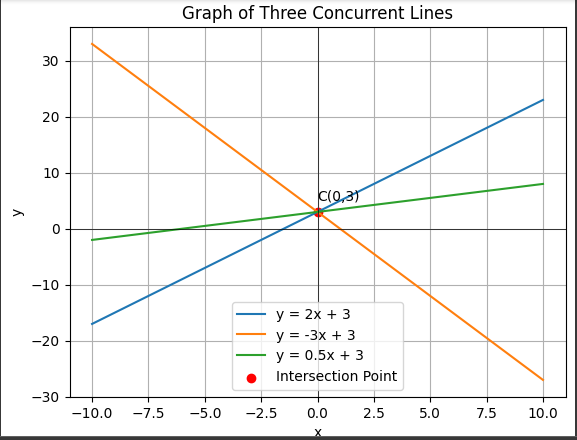
\includegraphics[width=\columnwidth]{concurrent.png}
    \caption{Straight Lines}
    \label{fig:concurrent.png}
\end{figure}
\end{enumerate}
\end{document} 
